\chapter{Implementación del sistema basado en IoT}\label{cap: }

\addcontentsline{toc}{section}{Introducción}
        \textbf{\Large Introducción}\newline
        ...

\section{Descripción técnica capa de percepción}

Como se analizaba en el epígrafe \ref{subsec:capa_percepcion} la capa de percepción va caracterizada por la presencia del microcontrolador y los sensores que, en conjunto forman los nodos, siendo estos los
encargados de la captura de los datos del medio.\\

Los nodos están diseñados sobre una placa de circuito impreso PCB (figura \ref{imag:pcb_nodo}).

\begin{figure}[H]
    \centering
    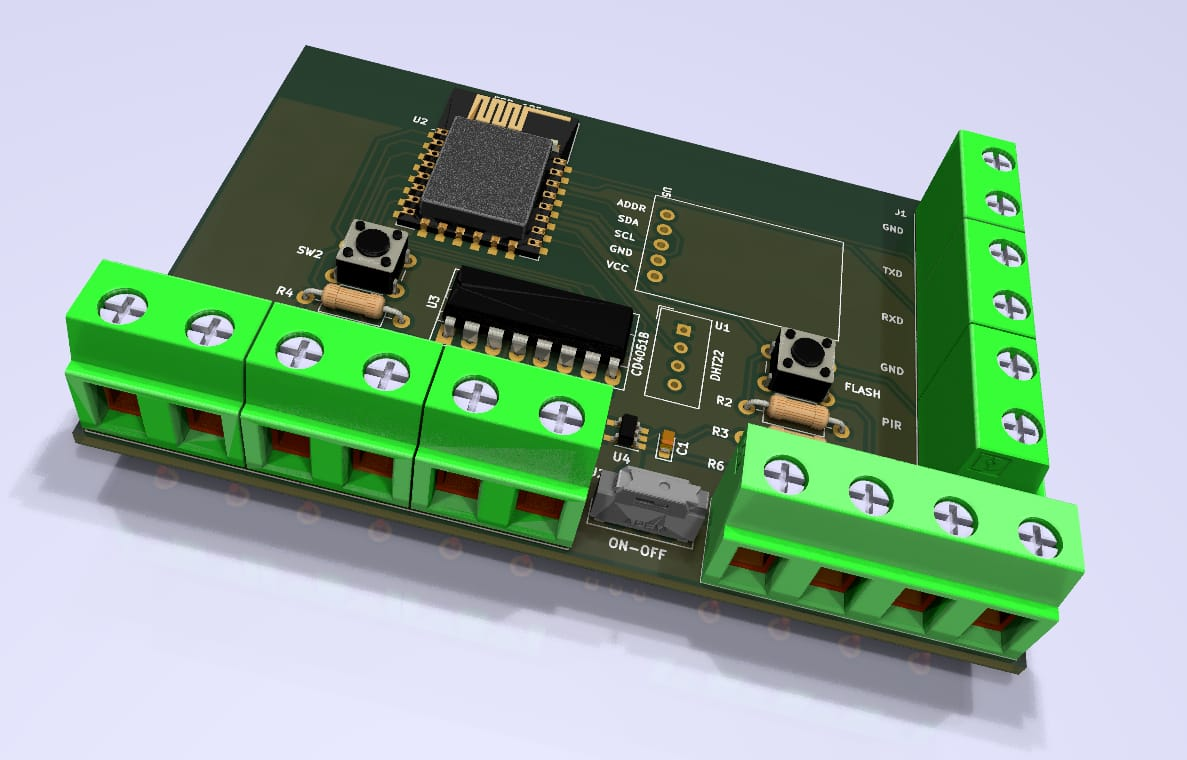
\includegraphics[width=7cm, height=5cm]{imagenes/vista 3D.jpg}
    \caption{PCB Nodo}
    \subcaption*{Fuente: Elavoración propia}
    \label{imag:pcb_nodo}
\end{figure}

\textbf{¿Por qué esta placa y no un Arduino o un NodeMcu?}

Al hablar de un microcontrolador como Arduino o NodeMcu se hace referencia a las posibilidades que brindan en cuanto a disponibilidad de pines GPIO. 

En el caso de un microcontrolador Arduino, dígase Arduino UNO, NANO, Arduino Micro ... 

Ahora, ¿por qué no se tomó ninguno de estos?

\begin{figure}[H]
    \centering
    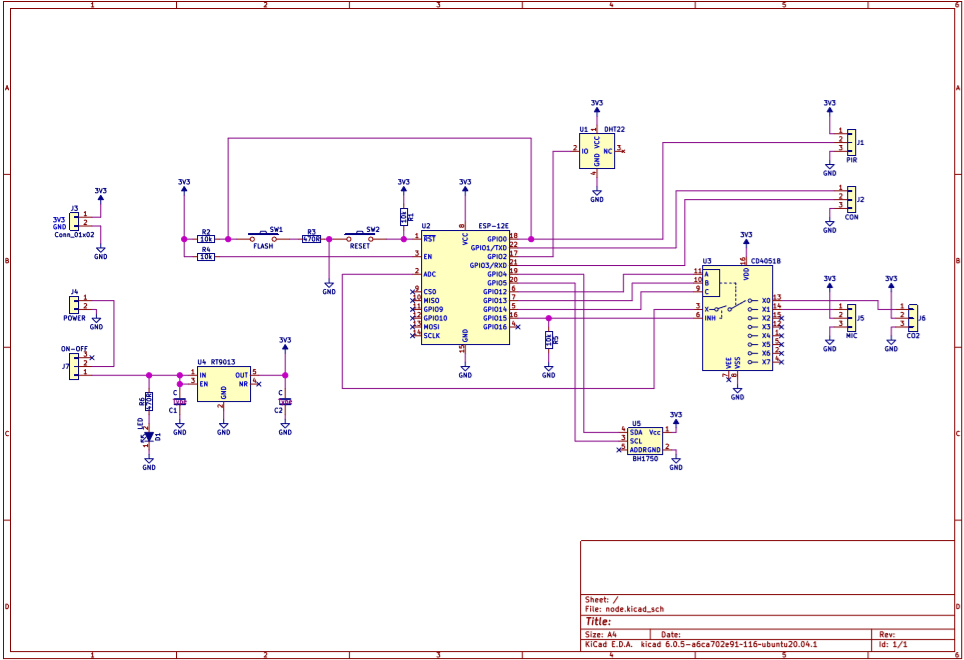
\includegraphics[width=12cm, height=8cm]{imagenes/esquematico nodo.jpg}
    \caption{Esquematico del circuito}
    \subcaption*{Fuente: Elavoración propia}
    \label{imag:esquematico_nodo}
\end{figure}

A continuación se describen por partes los elementos que componen dichos nodos.


\subsection{Microcontrolador} \label{sec: microcontrolador}

    Un microcontrolador (MCU) es un circuito integrado programable, capaz de ejecutar las órdenes grabadas en su memoria. Está compuesto de varios bloques funcionales, los cuales cumplen una tarea específica. Un microcontrolador incluye en su interior las tres principales unidades funcionales de una computadora: unidad central de procesamiento, memoria y periféricos de entrada/salida.\\

    El módulo WiFi ESP-12F fue desarrollado por Ai-Thinker Technology. El procesador central ESP8266 integra el micro MCU de 32 bits de potencia ultrabaja Tensilica L106 líder en la industria en un paquete pequeño con modo Lite de 16 bits, velocidad de reloj Admite 80 MHz y 160 MHz, admite RTOS e integra Wi-Fi MAC /BB/RF/PA/LNA.\\

    El módulo WiFi ESP-12F es compatible con el protocolo estándar IEEE802.11 b/g/n, una pila completa de protocolos TCP/IP. Los usuarios pueden usar este módulo para agregar capacidades de red a los dispositivos existentes o para construir controladores de red separados.

    El ESP8266 es un SOC inalámbrico de alto rendimiento que ofrece la máxima utilidad al menor costo y posibilidades ilimitadas para integrar la funcionalidad WiFi en otros sistemas.
    
    El ESP8266 es una solución de red Wi-Fi completa y autónoma que puede funcionar de forma independiente o como un esclavo que se ejecuta en otras MCU anfitrionas. El ESP8266 es capaz de arrancar directamente desde una memoria flash externa cuando está alimentado por una aplicación y es el único procesador de aplicaciones en el dispositivo. El caché incorporado ayuda a mejorar el rendimiento del sistema y reduce los requisitos de memoria.\\

    En otro caso, el ESP8266 se encarga del acceso inalámbrico a Internet. Cuando se trata de la tarea del adaptador WiFi, se puede agregar a cualquier diseño basado en un microcontrolador. La conexión es simple y fácil, solo por interfaz SPI/SDIO o puerto I2C/UART.

    Las potentes capacidades de almacenamiento y procesamiento en chip del ESP8266 le permiten integrar sensores y otros dispositivos específicos de la aplicación a través del puerto GPIO, lo que minimiza los recursos del sistema durante un desarrollo y una operación iniciales mínimos \cite{esp12}.\\

    El microcontrolador ESP-12F de Ai-Thinker (Figura \ref{imag:esp-12F}), basado en ESP8266.

    \begin{figure}[H]
        \centering
        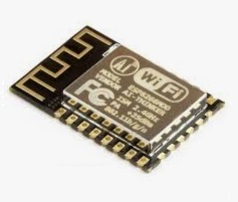
\includegraphics[width=4cm, height=4cm]{imagenes/esp-12F.jpeg}
        \caption{ESP-12F}
        \label{imag:esp-12F}
    \end{figure}

    \textbf{Características}

    \begin{itemize}
        \item The smallest 802.11b/g/n Wi-Fi SOC module
        \item Low power 32-bit CPU, can also serve as the application processor
        \item Up to 160MHz clock speed
        \item Built-in 10 bit high precision ADC
        \item Supports UART/GPIO/IIC/PWM/ADC
        \item SMD-22 package for easy welding
        \item Integrated Wi-Fi MAC/BB/RF/PA/LNA
        \item Support multiple sleep patterns. Deep sleep current as low as 20uA
        \item UART baud rate up to 4Mbps
        \item Embedded LWIP protocol stack
        \item Supports STA/AP/STA + AP operation mode
        \item Support Smart Config/AirKiss technology
        \item Supports remote firmware upgrade (FOTA)
        \item General AT commands can be used quickly
    \end{itemize}

    \begin{figure}[H]
        \centering
        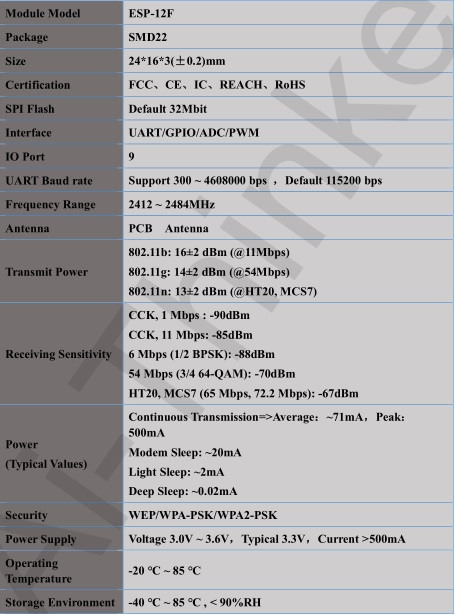
\includegraphics[width=10cm, height=13cm]{imagenes/esp-12F especificaciones.jpg}
        \caption{Especificaciones ESP-12F}
        \subcaption*{Fuente: Datasheet fabricante}
        \label{imag:esp-12F_especificaciones}
    \end{figure}

    
    \begin{figure}[H]
        \centering
        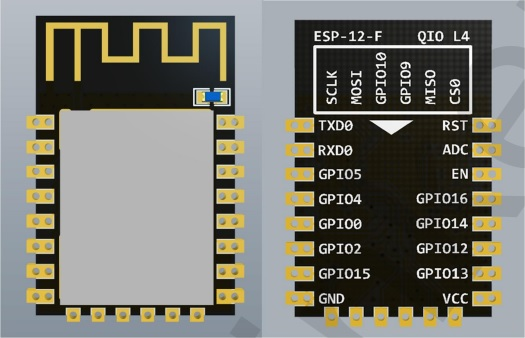
\includegraphics[width=6cm, height=4cm]{imagenes/esp-12F pinout.jpg}
        \caption{ESP-12F Pinout}
        \subcaption*{Fuente: Datasheet fabricante}
        \label{imag:esp-12F_pinout}
    \end{figure}

    \begin{figure}[H]
        \centering
        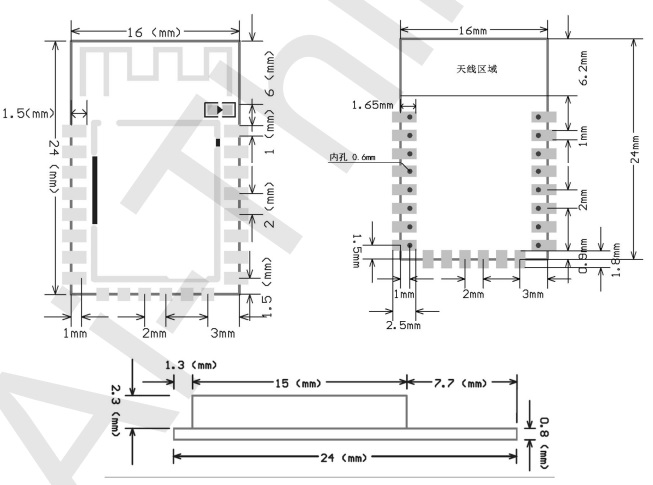
\includegraphics[width=10cm, height=7cm]{imagenes/esp-12F dimensiones.jpg}
        \caption{ESP-12F Dimensiones}
        \subcaption*{Fuente: Datasheet fabricante}
        \label{imag:esp-12F_dimensiones}
    \end{figure}

    \vspace{4cm}

    %Dentro de la familia de los ESP se encuentra el NodeMCU. Este microcontrolador (Imagen \ref{imag:nodemcu}) será el encargado de recibir los datos de los sensores y organizarlos en función de su continua transmisión hacia el concentrador.\\

    %\begin{figure}[h]
    %    \centering
    %    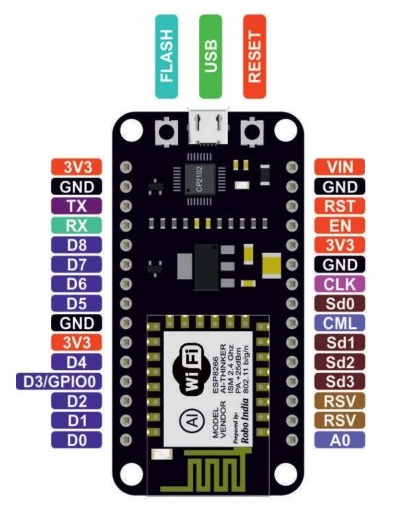
\includegraphics[width=5.5cm, height=6cm]{imagenes/nodemcu0.jpg}
    %    \caption{NodeMcu Vendor}
    %    \label{imag:nodemcu}
    %\end{figure}
    
    
    %NodeMCU es una pequeña placa Wifi compatible con Arduino, lista para usar en cualquier proyecto IoT. Está montada alrededor del microcontrolador ESP8266 y expone todos sus pines en los laterales. Además, ofrece más ventajas como la incorporación de un regulador de tensión integrado, así como un puerto USB de programación. Se puede programar con LUA o mediante el IDE de Arduino.\\

    %Dispone de una extensa comunidad y documentación que permitirá conectar el proyecto mediante conexión Wifi.

    %\textbf{Características}
    %\begin{itemize}
    %    \item Procesador: ESP8266 a 80MHz (3.3V) (ESP-12E).
    %    \item 4MB de memoria FLASH (32 MBit).
    %    \item WiFi 802.11 b/g/n.
    %    \item Regulador 3.3V integrado (500mA).
    %    \item Conversor USB-Serial CH340G.
    %    \item Función Auto-reset.
    %    \item 9 pines GPIO con I2C y SPI.
    %    \item 1 entrada analógica (1.0V max).
    %    \item 4 agujeros de montaje (3mm).
    %    \item Entrada alimentación externa VIN (20V max).
    %\end{itemize}

    \newpage

\subsection{Sensores} \label{sec: sensores}

    La secuencia de sensores pertenecientes al sistema es selecta, puesto que se tomaron los sensores teniendo en cuenta varios factores:

    \begin{itemize}
        \item Variable a medir
        \item Rango de operación
        \item Precisión
        \item Voltaje de alimentación
        \item Corriente de alimentación
        \item Precio
    \end{itemize}

    \vspace{1cm}

En la siguiente tabla se relacionan los mismos.

\begin{table}[H]
    \centering
    \caption{Relación sensores}
    \subcaption*{Fuente: Elaboración propia}
    \begin{tabular}{|c|c|c|cccc|}
    \hline
    \rowcolor[HTML]{9698ED} 
    \cellcolor[HTML]{9698ED}                      & \cellcolor[HTML]{9698ED}                                        & \cellcolor[HTML]{9698ED}                         & \multicolumn{4}{c|}{\cellcolor[HTML]{9698ED}Características}                                                                                                                                                                                                                          \\ \cline{4-7} 
    \rowcolor[HTML]{9698ED} 
    \multirow{-2}{*}{\cellcolor[HTML]{9698ED}No.} & \multirow{-2}{*}{\cellcolor[HTML]{9698ED}Variable}              & \multirow{-2}{*}{\cellcolor[HTML]{9698ED}Nombre} & \multicolumn{1}{c|}{\cellcolor[HTML]{9698ED}Rango}                                           & \multicolumn{1}{c|}{\cellcolor[HTML]{9698ED}Precisión} & \multicolumn{1}{c|}{\cellcolor[HTML]{9698ED}\begin{tabular}[c]{@{}c@{}}Voltaje\\ alimentación\end{tabular}} & Corriente       \\ \hline
    1                                             & \begin{tabular}[c]{@{}c@{}}Temperatura y\\ Humedad\end{tabular} & DHT22                                            & \multicolumn{1}{c|}{\begin{tabular}[c]{@{}c@{}}De - 40 a 80°C y\\ De 0 a 100RH\end{tabular}} & \multicolumn{1}{c|}{5\%}                               & \multicolumn{1}{c|}{De 3v a 6v}                                                                             & 2.5mA           \\ \hline
    2                                             & CO2                                                             & MH-Z19C                                          & \multicolumn{1}{c|}{\begin{tabular}[c]{@{}c@{}}De 400ppm a\\ 5000ppm\end{tabular}}           & \multicolumn{1}{c|}{5\%}                               & \multicolumn{1}{c|}{5v}                                                                                     & \textless{}40mA \\ \hline
    3                                             & Vibración                                                       & M0168                                            & \multicolumn{1}{c|}{\begin{tabular}[c]{@{}c@{}}Salida analógica\\ (0-1024)\end{tabular}}     & \multicolumn{1}{c|}{2\%}                               & \multicolumn{1}{c|}{De 3.3v a 5v}                                                                           & \textless{}10mA \\ \hline
    4                                             & Polución                                                        & SDS011                                           & \multicolumn{1}{c|}{\begin{tabular}[c]{@{}c@{}}De 0.0 a\\ 999.9ugm3\end{tabular}}            & \multicolumn{1}{c|}{10\%}                              & \multicolumn{1}{c|}{5v}                                                                                     & 100mA           \\ \hline
                                                  &                                                                 & LDR                                              & \multicolumn{1}{c|}{}                                                                        & \multicolumn{1}{c|}{}                                  & \multicolumn{1}{c|}{5v}                                                                                     & 10mA            \\ \cline{3-7} 
    \multirow{-2}{*}{5}                           & \multirow{-2}{*}{Luz}                                           & BH1750                                           & \multicolumn{1}{c|}{De 1 a 65535 lx}                                                         & \multicolumn{1}{c|}{20\%}                              & \multicolumn{1}{c|}{De 2.4v a 3.6v}                                                                         & 0.12mA          \\ \hline
    \end{tabular}
    \label{tab:relacion_sensores}
\end{table}

Se tomaron precios de referencia de los sensores de las páginas oficiales de compras online Amazon y Aliexpress para tener una idea del coste de montaje de los nodos.\\

\begin{table}[H]
    \centering
    \caption{Relación precios de referencia}
    \subcaption*{Fuente: Elavoración propia}
    \begin{tabular}{|c|c|c|}
    \hline
    \textbf{Sensor} & \textbf{Precio Amazon (U)} & \textbf{Precio Aliexpress (U)} \\ \hline
    DHT22           & 13.69 – 16.99 \$           & 2 – 4 \$                       \\ \hline
    MH-Z19C         & -                          & 16.99 \$                       \\ \hline
    M0168           & -                          & 0.31 – 1.34 \$                 \\ \hline
    SDS011          & 14.62 \$                   & 17.64 \$                       \\ \hline
    LDR             & 14.50 \$                   & 0.82 \$                        \\ \hline
    BH1750          & -                          & 8.46 \$                        \\ \hline
    \end{tabular}
    \label{tab: precios_referencia}
\end{table}

\subsection{Descripción sensores} \label{subsec: descripcion_sensores}

\addcontentsline{toc}{subsection}{\hspace{1.3cm}2.2.1.1\hspace{5mm}Sensor DHT22}
        \textbf{2.2.1.1\hspace{5mm}Sensor DHT22}

  \begin{figure}[H]
      \centering
      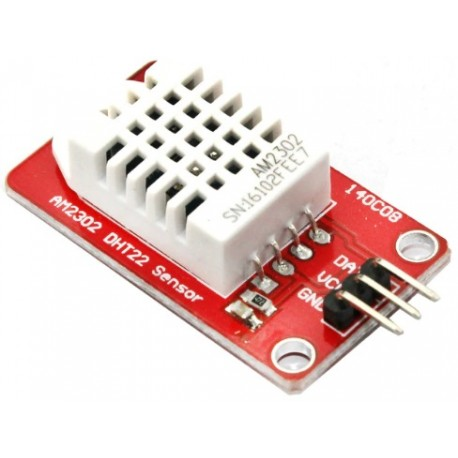
\includegraphics[width=5cm, height=5cm]{imagenes/dht22.jpg}
      \caption{Sensor DHT22}
      \subcaption*{Fuente: Datasheet fabricante}
      \label{imag:dht22}
   \end{figure}
   
El DHT22 (AM2302) es un sensor digital de temperatura y humedad relativa de buen rendimiento y de bajo costo. Integra un sensor capacitivo de humedad y un termistor para medir el aire circundante, y muestra los datos mediante una señal digital en el pin de datos (no posee salida analógica).\\

\begin{figure}[H]
    \centering
    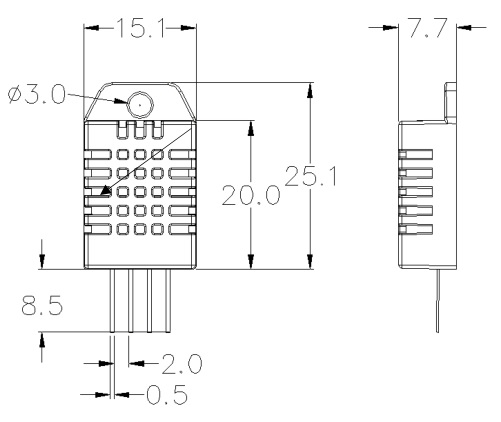
\includegraphics[width=8cm, height=6cm]{imagenes/dht22 dimensiones.jpg}
    \caption{Dimensiones sensor DHT22}
    \subcaption*{Fuente: Datasheet fabricante}
    \label{imag:dimensiones_dht22}
\end{figure}

\vspace{1cm}

\addcontentsline{toc}{subsection}{\hspace{1.3cm}2.2.1.2\hspace{5mm}Sensor MZ-Z19C}
        \textbf{2.2.1.2\hspace{5mm}Sensor MZ-Z19C}

\begin{figure}[H]
      \centering
      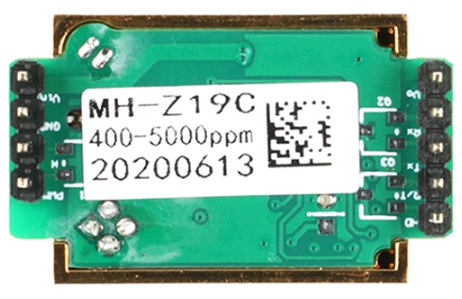
\includegraphics[width=5cm, height=3cm]{imagenes/mh-z19c.png}
      \caption{Sensor MH-Z19C}
      \label{imag:mh-z19c}
   \end{figure}

El sensor de gas de dióxido de carbono MH-Z19C es un pequeño sensor inteligente de uso general que utiliza el principio del infrarrojo no disperso (NDIR) para detectar la presencia de CO2 en el aire.\\

\textbf{Otros datos}
\begin{itemize}
    \item Señal de salida: UART(TTL)
    \item Tiempo de precalentamiento: 60 segundos
    \item Temperatura de operación: De -10 a 50°C
    \item Humedad de operación: De 0 - 95 por ciento RH
    \item Dimensiones: aprox. 39 x 20 x 9 mm
    \item Tipo de conector: JST ZH de 7 pines
\end{itemize}

\vspace{0.5cm}

\addcontentsline{toc}{subsection}{\hspace{1.3cm}2.2.1.3\hspace{5mm}Sensor M0168}
        \textbf{2.2.1.3\hspace{5mm}Sensor M0168}

\begin{figure}[H]
      \centering
      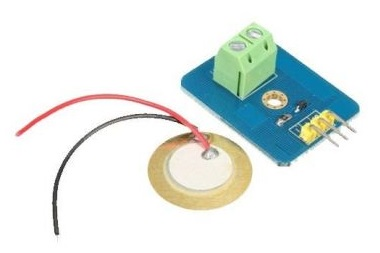
\includegraphics[width=6.5cm, height=5cm]{imagenes/sensor-piezoelectrico.jpg}
      \caption{Sensor piezoeléctrico M0168}
      \label{imag:M0168}
   \end{figure}

En este sensor piezoeléctrico cuando el choque de la cerámica con la lámina metálica genera una señal eléctrica, esta señal analógica es la recibida por los pines analógicos de microcontroladores.\\

\textbf{Especificaciones Técnicas}

\begin{itemize}
    \item Voltaje de trabajo: 3.3V o 5V
    \item Corriente de trabajo: 1mA
    \item Rango de temperatura de funcionamiento: -10 ~ +70
    \item Interfaz Tipo: salida analógica
    \item Tamaño del artículo: 30mm x 23mm
\end{itemize}

\newpage

\addcontentsline{toc}{subsection}{\hspace{1.3cm}2.2.1.4\hspace{5mm}Sensor SDS011}
        \textbf{2.2.1.4\hspace{5mm}Sensor SDS011}

\vspace{1cm}

\begin{figure}[H]
      \centering
      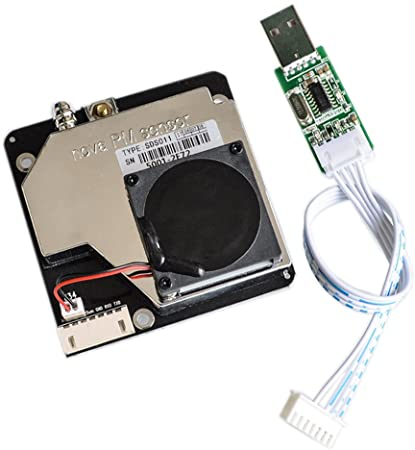
\includegraphics[width=4.5cm, height=4.5cm]{imagenes/Sensor SDS011.jpg}
      \caption{Sensor SDS011}
      \label{imag:SDS011}
   \end{figure}

Se basa en el principio de dispersión láser: se puede inducir la dispersión de la luz cuando las partículas atraviesan el área de detección. La luz dispersa se transforma en señales eléctricas, después estas señales serán amplificadas y procesadas. El número y el diámetro de las partículas se pueden obtener mediante análisis porque la forma de onda tiene ciertas relaciones con el diámetro de las partículas.\\

\textbf{Otros datos}

\begin{itemize}
    \item Corriente del sueño: 2mA
    \item Frecuencia de muestreo serie: 1 segundo
    \item Resolución diámetro de partículas: <= 0.3um
    \item Rango de temperatura: -20 a 50°C
    \item Tamaño físico: 71mm x 70mm x 23mm 
\end{itemize}

\vspace{5cm}

\addcontentsline{toc}{subsection}{\hspace{1.3cm}2.2.1.5\hspace{5mm}Sensor LDR}
        \textbf{2.2.1.5\hspace{5mm}Sensor LDR}\newline

\begin{figure}[H]
      \centering
      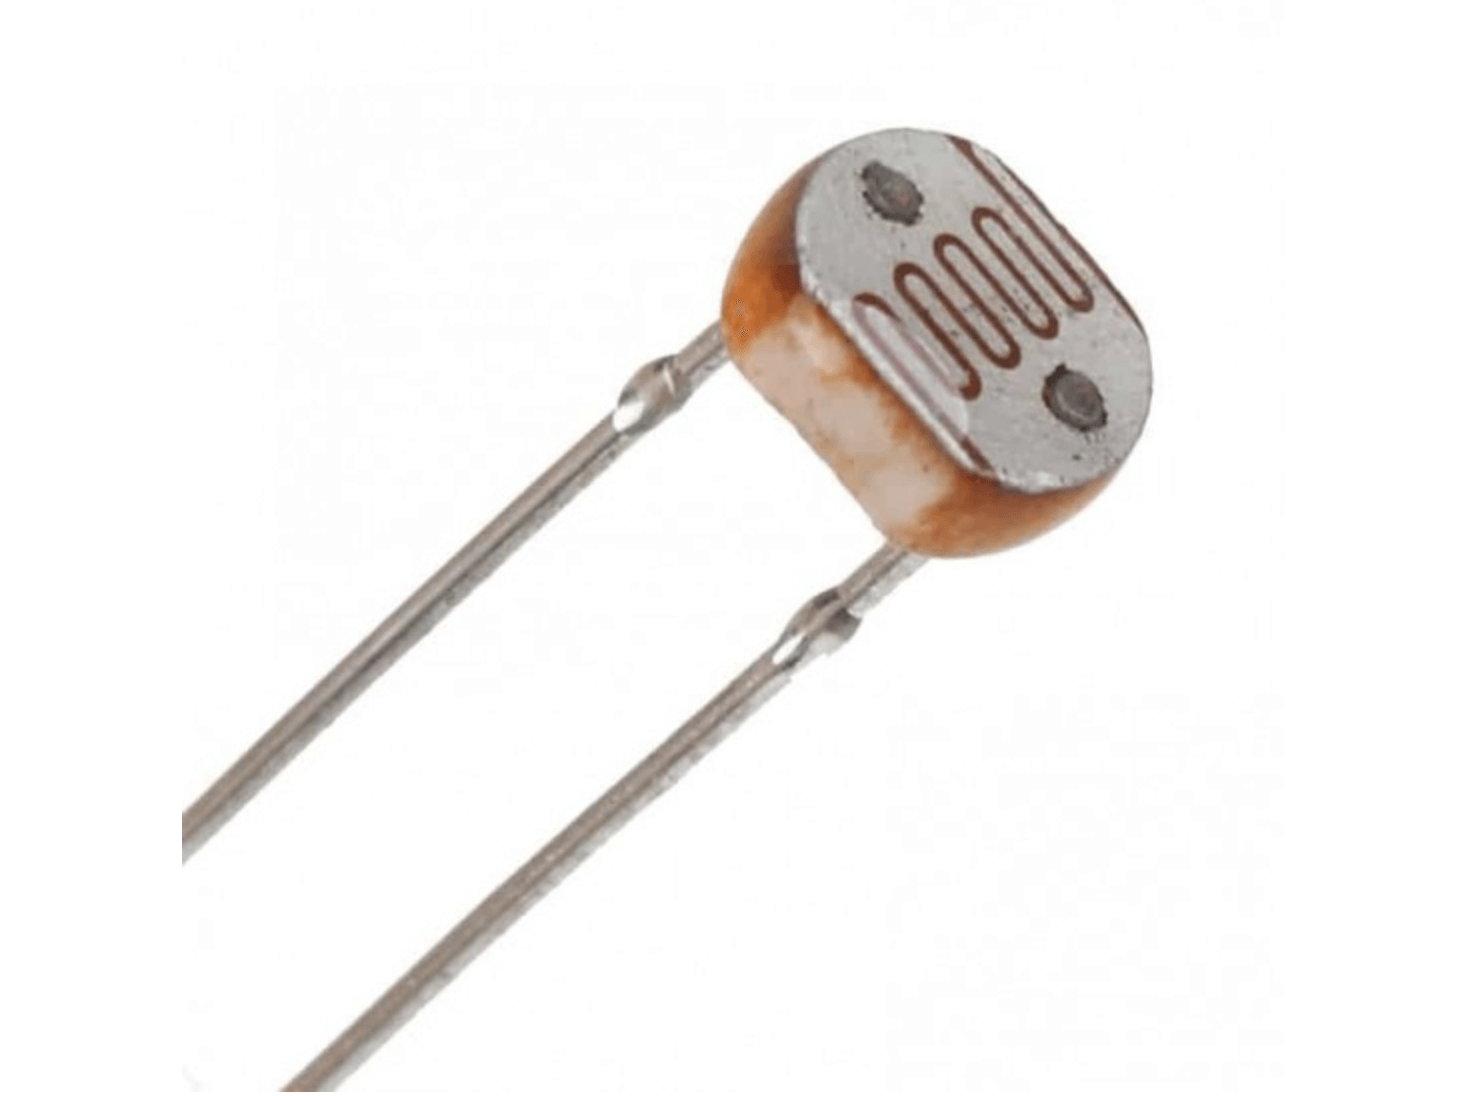
\includegraphics[width=5.5cm, height=4cm]{imagenes/sensor LDR.png}
      \caption{Sensor LDR}
      \label{imag:LDR}
   \end{figure}

Una fotorresistencia es un componente electrónico cuya resistencia disminuye con el aumento de la intensidad de la luz incidente. Puede también ser llamado fotorresistor, fotoconductor, célula fotoeléctrica o resistor dependiente de la luz, cuyas siglas, LDR, se originan de su nombre en inglés light-dependent resistor.\\

\begin{figure}[H]
    \centering
    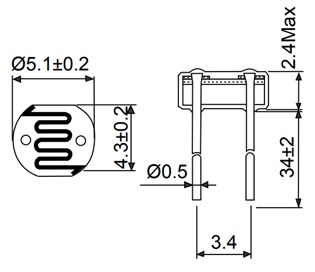
\includegraphics[width=4.5cm, height=4cm]{imagenes/ldr.jpg}
    \caption{Sensor LDR}
    \subcaption*{Fuente: Datasheet fabricante}
    \label{imag:dimensiones LDR}
 \end{figure}

\vspace{0.5cm}

\addcontentsline{toc}{subsection}{\hspace{1.3cm}2.2.1.6\hspace{5mm}Sensor BH1750}
        \textbf{2.2.1.6\hspace{5mm}Sensor BH1750}\newline

El Módulo BH1750 es un sensor de iluminación digital para medición de flujo luminoso (iluminancia) de la empresa Rohm Semiconductor. Componente que posee dentro de su arquitectura interna, un conversor análogo digital (ADC) de 16 bits con una salida digital de formato I2C, que facilita la integración con microcontroladores o sistemas embebidos diversos. Este módulo entrega la intensidad luminosa directamente en unidades de Lux que es equivalente a Lumen/m2.\\

\begin{figure}[H]
    \centering
    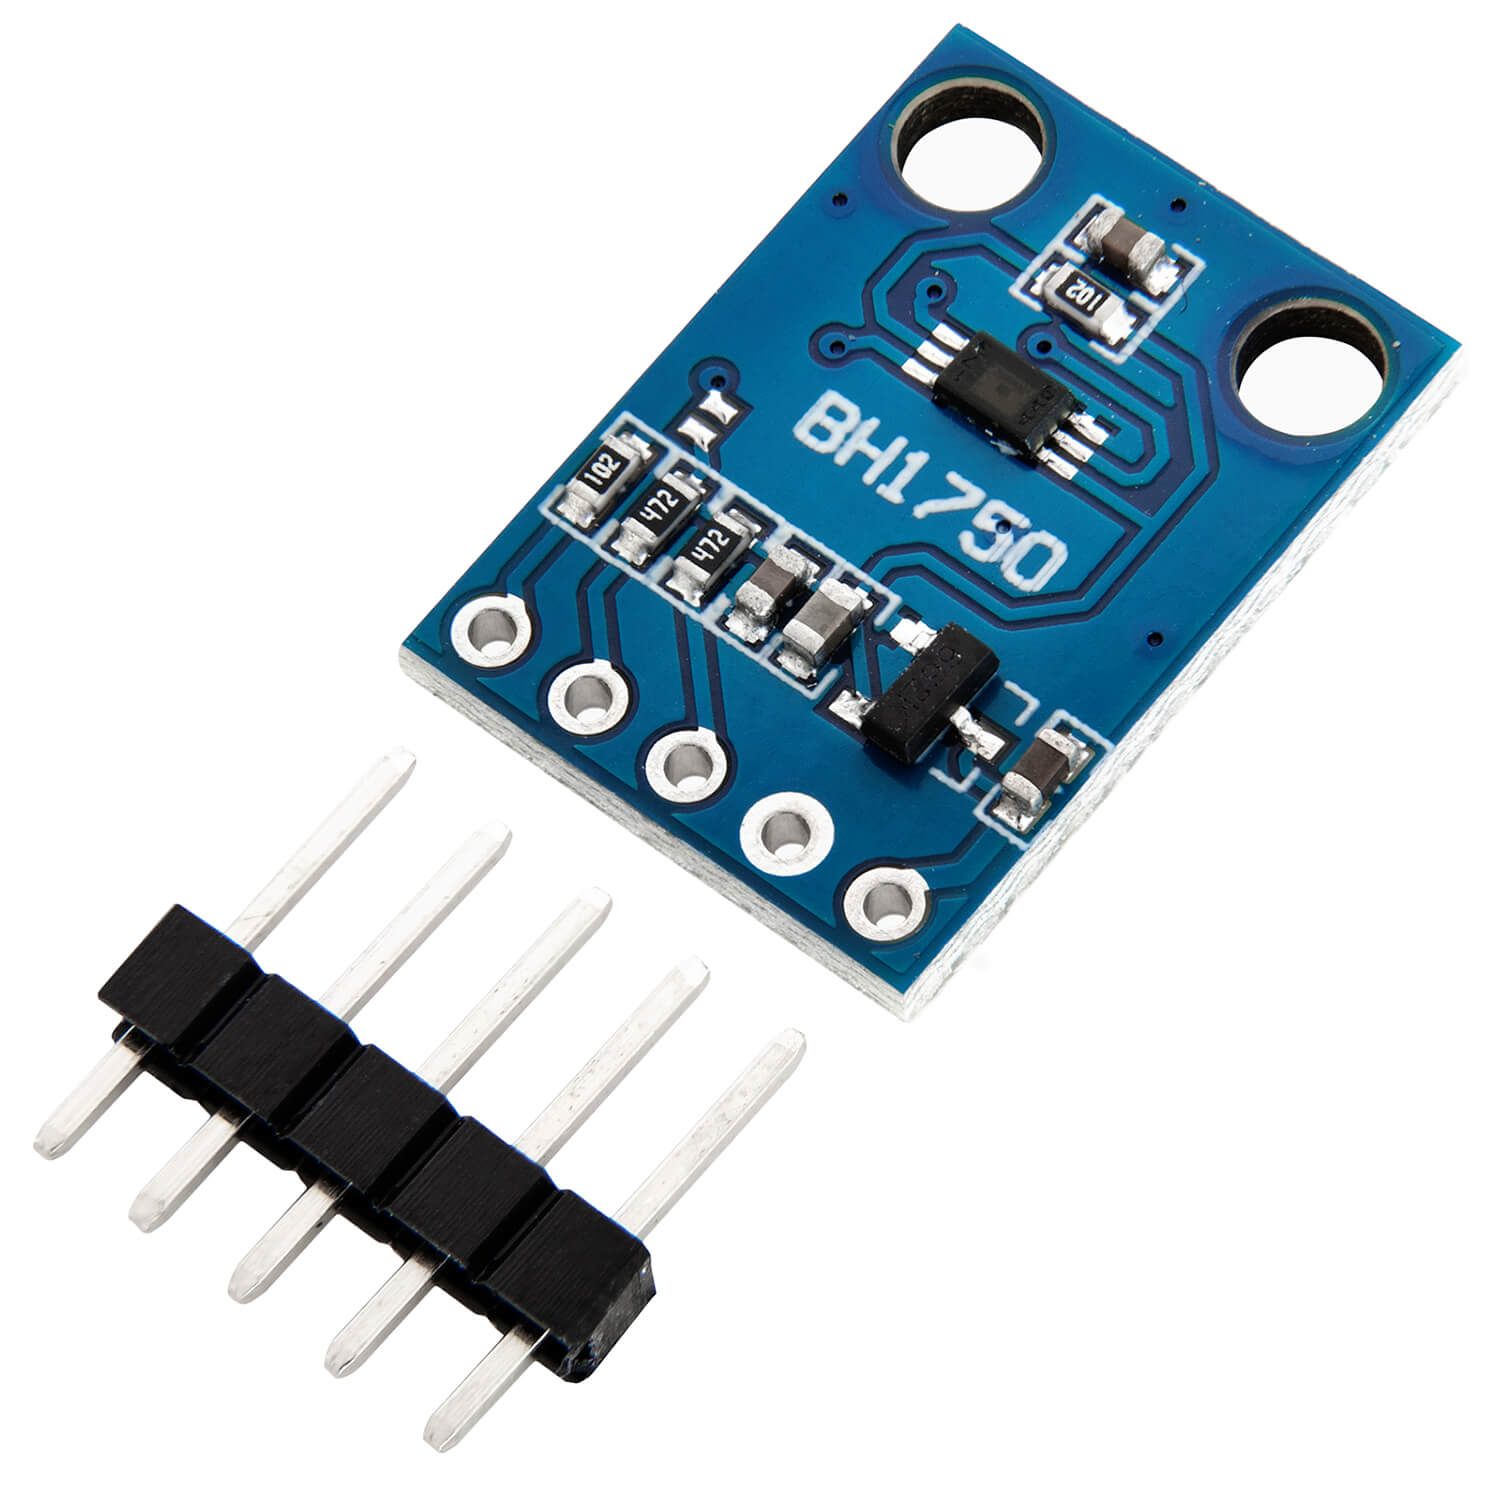
\includegraphics[width=5cm, height=4cm]{imagenes/Sensor BH1750.jpg}
    \caption{Sensor BH1750}
    \label{imag:BH1750}
 \end{figure}

\textbf{Otros datos}

\begin{itemize}
    \item Interfaz Digital: I2C
    \item Frecuencia máxima de transmisión: 400kHZ
    \item Temperatura de operación: Desde -40°C hasta 85°C
\end{itemize}

Para su correcto funcionamiento, este sensor debe ir acompañado de una serie de componentes electrónicos para su acondicionamiento.
En la figura \ref{imag:acondicionamiento_BH1750} se puede observar el acondicionamiento brindado por el fabricante.

\begin{figure}[H]
    \centering
    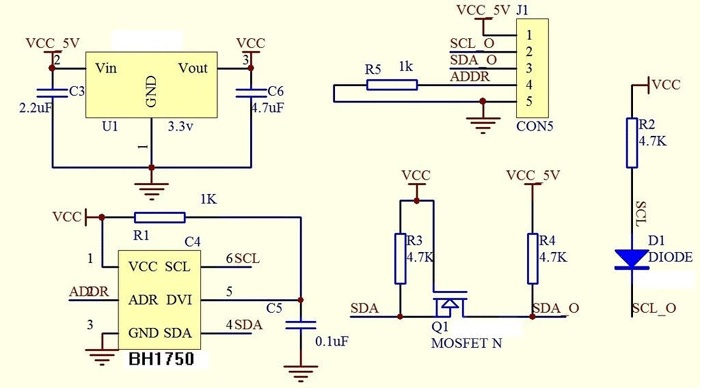
\includegraphics[width=11cm, height=7cm]{imagenes/acondicionamientos sensor BH1750.jpg}
    \caption{Acondicionamiento sensor BH1750}
    \subcaption*{Fuente: Datasheet fabricante}
    \label{imag:acondicionamiento_BH1750}
\end{figure}

\vspace{1cm}

\subsection{Alimentación}

\textbf{Regulador LDO RT9013.}\newline

El RT9013 es un regulador LDO de 500 mA de alto rendimiento que ofrece PSRR extremadamente alto y caída ultrabaja. Ideal para aplicaciones inalámbricas y de RF portátiles con requisitos exigentes de rendimiento y espacio.\\

La corriente de reposo RT9013 es tan baja como 25uA, lo que prolonga aún más la vida útil de la batería. El RT9013 también funciona con condensadores cerámicos de baja ESR, lo que reduce la cantidad de espacio de placa necesario para las aplicaciones de energía, lo que es fundamental en los dispositivos inalámbricos de mano.\\

El RT9013 consume 0.7uA típicos en modo de apagado y tiene un tiempo de encendido rápido de menos de 40us. Las otras características incluyen voltaje de caída ultrabajo, alta precisión de salida, protección de limitación de corriente y alta relación de rechazo de ondulación. Disponible en el paquete SC-82, SOT-23-5, SC-70-5 y WDFN-6L 2x2.\\

\textbf{Características}

\begin{itemize}
    \item Amplios rangos de voltaje de operación: 2.2V a 5.5V
    \item Caída baja: 250mV a 500mA
    \item Ruido ultrabajo para aplicaciones de RF
    \item Respuesta ultrarrápida en transitorios de línea/carga
    \item Protección de limitación de corriente
    \item Protección de apagado térmico
    \item Tasa de rechazo de fuente de alimentación alta
    \item A la salida solo se requiere 1 uF de condensador para la estabilidad
    \item Entrada de apagado controlado por lógica TTL
\end{itemize}

\vspace{1cm}

\begin{figure}[H]
    \centering
    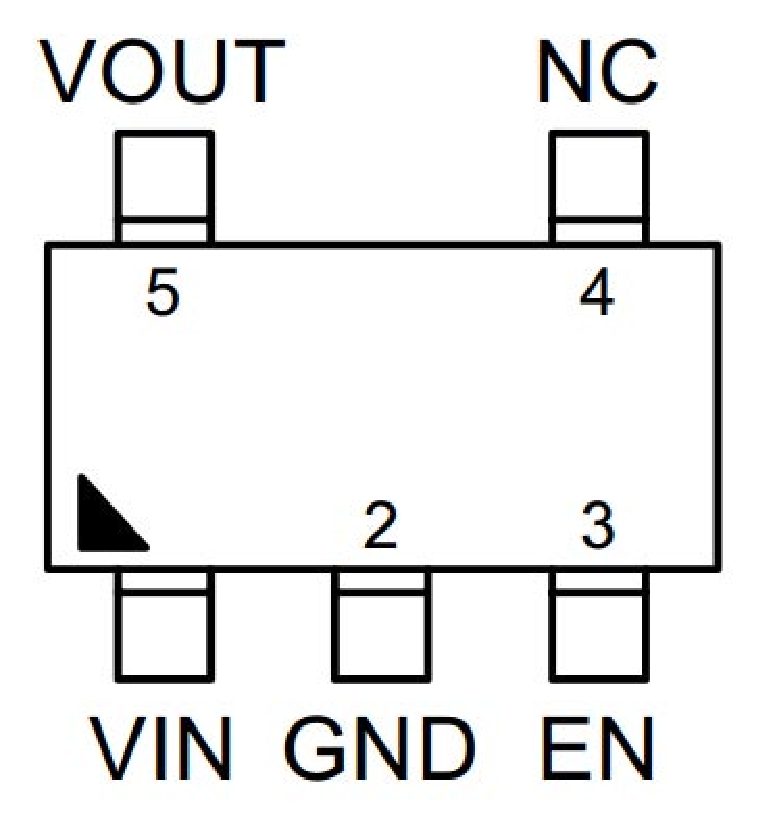
\includegraphics[width=5.5cm, height=6cm]{imagenes/esquematico RT9013.pdf}
    \caption{Configuración de pines}
    \subcaption*{Fuente: Datasheet fabricante}
    \label{imag:pines_RT9013}
\end{figure}

\begin{figure}[H]
    \centering
    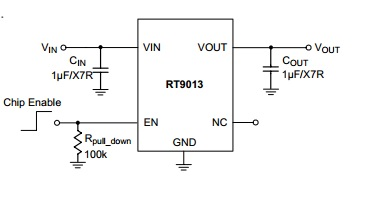
\includegraphics[width=12cm, height=7cm]{imagenes/acondicionamiento RT9013.jpg}
    \caption{Acondicionamiento}
    \subcaption*{Fuente: Datasheet fabricante}
    \label{imag:acondicionamiento_RT9013}
\end{figure}

\newpage

\section{Condiciones medioambientales...} \label{sec: condiciones_medioambientales}


    \begin{figure}[H]
        \centering
        \includegraphics[width=16cm, height=5cm]{imagenes/gráfica_comparativa_variables_medioambientales.png}
        \caption{Correlación de valores medioambientales}
        \subcaption*{Fuente: Elaboración propia}
        \label{imag:grafica_condiciones_medioambientales}
    \end{figure}


\addcontentsline{toc}{section}{Conclusiones}
        \textbf{\Large Conclusiones}\newline
